\documentclass[11pt,openany]{book}
\usepackage[]{graphicx}\usepackage[]{color}
%% maxwidth is the original width if it is less than linewidth
%% otherwise use linewidth (to make sure the graphics do not exceed the margin)
\makeatletter
\def\maxwidth{ %
  \ifdim\Gin@nat@width>\linewidth
    \linewidth
  \else
    \Gin@nat@width
  \fi
}
\makeatother

\definecolor{fgcolor}{rgb}{0.345, 0.345, 0.345}
\newcommand{\hlnum}[1]{\textcolor[rgb]{0.686,0.059,0.569}{#1}}%
\newcommand{\hlstr}[1]{\textcolor[rgb]{0.192,0.494,0.8}{#1}}%
\newcommand{\hlcom}[1]{\textcolor[rgb]{0.678,0.584,0.686}{\textit{#1}}}%
\newcommand{\hlopt}[1]{\textcolor[rgb]{0,0,0}{#1}}%
\newcommand{\hlstd}[1]{\textcolor[rgb]{0.345,0.345,0.345}{#1}}%
\newcommand{\hlkwa}[1]{\textcolor[rgb]{0.161,0.373,0.58}{\textbf{#1}}}%
\newcommand{\hlkwb}[1]{\textcolor[rgb]{0.69,0.353,0.396}{#1}}%
\newcommand{\hlkwc}[1]{\textcolor[rgb]{0.333,0.667,0.333}{#1}}%
\newcommand{\hlkwd}[1]{\textcolor[rgb]{0.737,0.353,0.396}{\textbf{#1}}}%
\let\hlipl\hlkwb

\usepackage{framed}
\makeatletter
\newenvironment{kframe}{%
 \def\at@end@of@kframe{}%
 \ifinner\ifhmode%
  \def\at@end@of@kframe{\end{minipage}}%
  \begin{minipage}{\columnwidth}%
 \fi\fi%
 \def\FrameCommand##1{\hskip\@totalleftmargin \hskip-\fboxsep
 \colorbox{shadecolor}{##1}\hskip-\fboxsep
     % There is no \\@totalrightmargin, so:
     \hskip-\linewidth \hskip-\@totalleftmargin \hskip\columnwidth}%
 \MakeFramed {\advance\hsize-\width
   \@totalleftmargin\z@ \linewidth\hsize
   \@setminipage}}%
 {\par\unskip\endMakeFramed%
 \at@end@of@kframe}
\makeatother

\definecolor{shadecolor}{rgb}{.97, .97, .97}
\definecolor{messagecolor}{rgb}{0, 0, 0}
\definecolor{warningcolor}{rgb}{1, 0, 1}
\definecolor{errorcolor}{rgb}{1, 0, 0}
\newenvironment{knitrout}{}{} % an empty environment to be redefined in TeX

\usepackage{alltt}
\newcommand{\SweaveOpts}[1]{}  % do not interfere with LaTeX
\newcommand{\SweaveInput}[1]{} % because they are not real TeX commands
\newcommand{\Sexpr}[1]{}       % will only be parsed by R


\usepackage[utf8]{inputenc} 
\usepackage{amssymb, amsmath, amsthm}
\usepackage{fullpage}
\usepackage{setspace}
\usepackage{graphicx}
\usepackage{natbib}
\usepackage{rotating}
\usepackage{caption}
\usepackage{subcaption}
\usepackage{multirow}
\usepackage{booktabs}
\usepackage{dcolumn}
\usepackage[grey]{quotchap}
\usepackage{xcolor}
\usepackage[left=1in, top=1in, right=1.5in, bottom=1in, headsep=.5in]
{geometry}
\usepackage{fancyhdr, blindtext}
\usepackage{diagbox}
\usepackage{hyperref} 
\usepackage{placeins}
\renewenvironment{knitrout}{\begin{singlespace}}{\end{singlespace}}
\newcommand*{\mybox}[2]{\colorbox{#1!30}{\parbox{.98\linewidth}{#2}}}
\newcommand*{\befehl}[1]{\texttt{\textbackslash #1}} % Added by 


\fancyhf{}
\fancyhead[LE]{\slshape \rightmark} 
\fancyhead[RE]{\thepage}
\fancyhead[RO]{\slshape \leftmark} 
\fancyhead[LO]{\thepage}
\renewcommand{\headrulewidth}{0.4pt}
\pagestyle{fancy}
%% new command for greybox
\long\def\greybox#1{%
    \newbox\contentbox%
    \newbox\bkgdbox%
    \setbox\contentbox\hbox to \hsize{%
        \vtop{
            \kern\columnsep
            \hbox to \hsize{%
                \kern\columnsep%
                \advance\hsize by -2\columnsep%
                \setlength{\textwidth}{\hsize}%
                \vbox{
                    \parskip=\baselineskip
                    \parindent=0bp
                    #1
                }%
                \kern\columnsep%
            }%
            \kern\columnsep%
        }%
    }%
    \setbox\bkgdbox\vbox{
        \pdfliteral{0.85 0.85 0.85 rg}
        \hrule width  \wd\contentbox %
               height \ht\contentbox %
               depth  \dp\contentbox
        \pdfliteral{0 0 0 rg}
    }%
    \wd\bkgdbox=0bp%
    \vbox{\hbox to \hsize{\box\bkgdbox\box\contentbox}}%
    \vskip\baselineskip%
}
%% make greybox (grbox) a float
\usepackage{float}
\newfloat{grbox}{thp}{lop}[section]
\floatname{grbox}{Grey Box}



\begin{document}






\chapter{Topics in Multiple Regression}


Thus far we have developed the basis for multiple OLS reression using matrix algebra, delved into the meaning of the estimated partial regression coefficient, and revisited the basis for hypothesis testing in OLS. In this chapter we turn to one of the key strengths of OLS: the robust flexibility of OLS for model specification. First we will discuss how to include binary variables (referred to as ``dummy variables") as IVs in an OLS model. Next ww will show you how to build on dummy variables to model their interactions with other variables in your model. Finally, we will address an alternative way to express the partial regression coefficients -- using standardized coefficients -- that permit you to compare the magnitudes of the estimated effects of your IVs even when they are measured on different scales. As has been our custom, the examples in this chapter are based on variable from the \texttt{tbur} data set.  

\section{Dummy Variables} 

Thus far, we have considered OLS models that include variables measured on interval level scales (or, in a pinch and with caution, ordinal scales). That is fine when we have variables for which we can develop valid and reliable interval (or ordinal) measures. But in the policy and social sciences we often want to include in our analysis concepts that do not readily admit to interval measure -- including many cases in which a variable has an ``on - off", or ``present - absent" quality. In other cases we want to include a concept that is essentially nominal in nature, such that an observation can be categorized as a subset but not measured on a ``high-low" or ``more-less" type of scale. In these instances we can utilize what is generally known as a dummy variable, but are also referred to as indicator variables, Boolean variables, or categorical variables.

\begin{grbox}
\greybox{\textbf{What the Heck are ``Dummy Variables"?}}

\begin{itemize}  
\item A dichotomous variable, with values of 0 and 1;
\item A value of 1 represents the presence of some quality, a zero its absence;
\item The 1s are compared to the 0s, who are known as the ``referent group";
\item Dummy variables are often thought of as a proxy for a qualitative variable.
\end{itemize}  
\end{grbox}

Dummy variables allow for tests of the differences in overall value of the $Y$ for different nominal groups in the data. They are akin to a difference of means test for the groups identified by the dummy variable. Dummy variables allow for comparisons between an included (the 1s) and an omitted (the 0s) group. Therefore, it is important to be clear about which group is omitted and serving as the ``comparison category." 

It is often the case that there are more than two groups, represented by a set of nominal categories. In that case, the variable will consist of two or more dummy variables, with 0/1 codes for each category except the referent group (which is omitted). Several examples of categorical variables that can be represented on multiple regression with dummy variables include:

\begin{itemize}
\item Experimental treatment and control groups (treatment=1, control=0)
\item Gender (male=1, female=0 or vice versa)
\item Race and ethnicity (a dummy for each group, with one omitted referent group)
\item Region of residence (dummy for each region with one omitted reference region)
\item Type of education (dummy for each type with omitted reference type)
\item Religious affiliation (dummy for each religious denomination with omitted reference)
\end{itemize}

The value of the dummy coefficient represents the estimated difference in $Y$ between the dummy group and the reference group. Because the estimated difference is the average over all of the $Y$ observations, the dummy is best understood as a change in the value of the intercept ($A$) for the ``dummied" group. This is illustrated in Figure \ref{fig:dum}. In this illustration, the value of $Y$  is a function of $X_1$ (a continuous variable) and $X_2$ (a dummy variable). When $X_2$ is equal to 0 (the referent case) the top regression line applies. When $X_2 = 1$, the value of $Y$ is reduced to the bottom line. In short, $X_2$ has a negative estimated partial regression coefficient represented by the difference in height between the two regression lines.

\begin{figure}
  \centering
  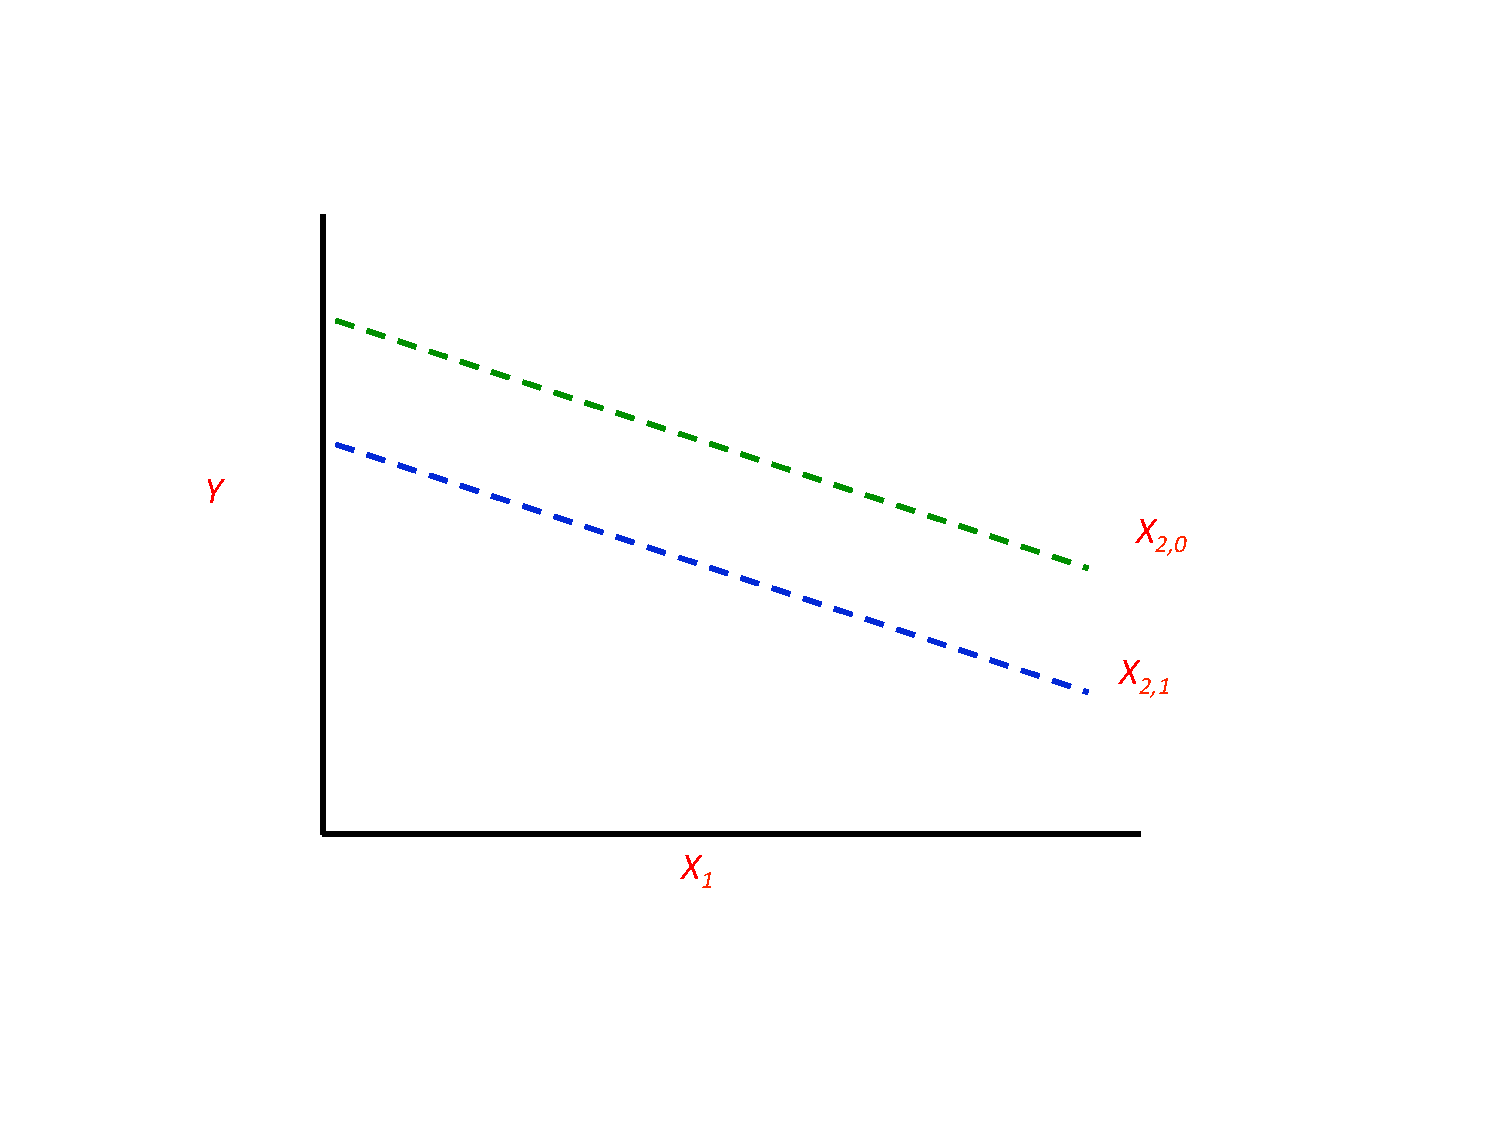
\includegraphics[width=5in]{../14_Topics/dummy.pdf}%filename
  \caption{Dummy Intercept Variables \label{fig:dum}}
\end{figure}

For a case with multiple nominal categories (e.g., region) the procedure is as follows: (a) determine which category will be assigned as the referent group; (b) create a dummy variable for each of the other categories. For example, if you are coding a dummy for four regions (North, South, East and West), you could designate the South as the referent group. Then you would create dummies for the other three regions. Then, all observations from
the North would get a value of 1 in the North dummy, and zeros in all others. Similarly, East and West observations would receive a 1 in their respective dummy category and zeros elsewhere. The observations from the South region would be given values of zero in all three categories. The interpretation of the partial regression coefficients for each of the three dummies would then be the estimated difference in $Y$ between observations from the North, East and West and those from the South.

Now let's walk through an example of an $R$ model with a dummy variable and the interpretation of that model. We will predict climate change risk using age, education, income, ideology, and ``gend", a dummy variable for gender for which 1 = male and 0 = female. 


\begin{knitrout}
\definecolor{shadecolor}{rgb}{0.969, 0.969, 0.969}\color{fgcolor}\begin{kframe}
\begin{alltt}
\hlstd{ols1} \hlkwb{<-} \hlkwd{lm}\hlstd{(glbcc_risk} \hlopt{~} \hlstd{age} \hlopt{+} \hlstd{education} \hlopt{+} \hlstd{income} \hlopt{+} \hlstd{ideol} \hlopt{+} \hlstd{gender,} \hlkwc{data} \hlstd{= ds.temp)}
\hlkwd{summary}\hlstd{(ols1)}
\end{alltt}
\begin{verbatim}
## 
## Call:
## lm(formula = glbcc_risk ~ age + education + income + ideol + 
##     gender, data = ds.temp)
## 
## Residuals:
##     Min      1Q  Median      3Q     Max 
## -8.8976 -1.6553  0.1982  1.4814  6.7046 
## 
## Coefficients:
##               Estimate Std. Error t value Pr(>|t|)    
## (Intercept)  1.094e+01  3.092e-01  35.379  < 2e-16 ***
## age         -4.062e-03  3.671e-03  -1.106  0.26865    
## education    6.653e-02  2.997e-02   2.220  0.02653 *  
## income      -2.372e-06  9.083e-07  -2.611  0.00908 ** 
## ideol       -1.032e+00  2.998e-02 -34.426  < 2e-16 ***
## gender      -2.221e-01  1.051e-01  -2.112  0.03475 *  
## ---
## Signif. codes:  0 '***' 0.001 '**' 0.01 '*' 0.05 '.' 0.1 ' ' 1
## 
## Residual standard error: 2.431 on 2265 degrees of freedom
## Multiple R-squared:  0.364,	Adjusted R-squared:  0.3626 
## F-statistic: 259.3 on 5 and 2265 DF,  p-value: < 2.2e-16
\end{verbatim}
\end{kframe}
\end{knitrout}
First note that the inclusion of the dummy variables doe not change the manner in which you interpret the other (non-dummy) variables in the model; the estimated partial regression coefficients for age, education, income and ideology should all be interpreted as described in the prior chapter. Note that the estimated partial regression coefficient for ``gender" is negative and statistically significant, indicating that males are less likely to be concerned about the environment than are females. The estimate indicates that, all else being equal, the average difference between men and women on the climate change risk scale is -0.2221178. 

%% in future editions I want to add a table showing how to code different kinds of dummy variables

\section{Interaction Effects}

Dummy variables can also be used to estimate the ways in which the effect of a variable differs across subsets of cases. These kinds of effects are generally called ``interactions".  When an interaction occurs, the effect of one $X$ is dependent on the value of another. Typically, an OLS model is additive, where the $B$'s are added together to predict $Y$; 

  $Y_i = A + BX_1 + BX_2 + BX_3 + BX_4 + E_i$. 
  
However, an interaction model has a multiplicative effect where two of the IVs are multiplied;

  $Y_i = A + BX_1 + BX_2 + BX_3 * BX_4 + E_i$. 

A ``slope dummy" is a special kind of interaction in which a dummy variable  is interacted with (multiplied by) a scale (ordinal or higher) variable. Suppose, for example, that you hypothesized that the effects of political of ideology on perceived risks of climate change were different for men and women. Perhaps men are more likely than women to consistently integrate ideology into climate change risk perceptions. In such a case, a dummy variable (0=women, 1=men) could be interacted with ideology (1=strong liberal, 7=strong conservative) to predict levels of perceived risk of climate change (0=no risk, 10=extreme risk).  If your hypothesized interaction was correct, you would observe the kind of pattern as shown in Figure \ref{fig:dumin}. 

\begin{figure}
  \centering
  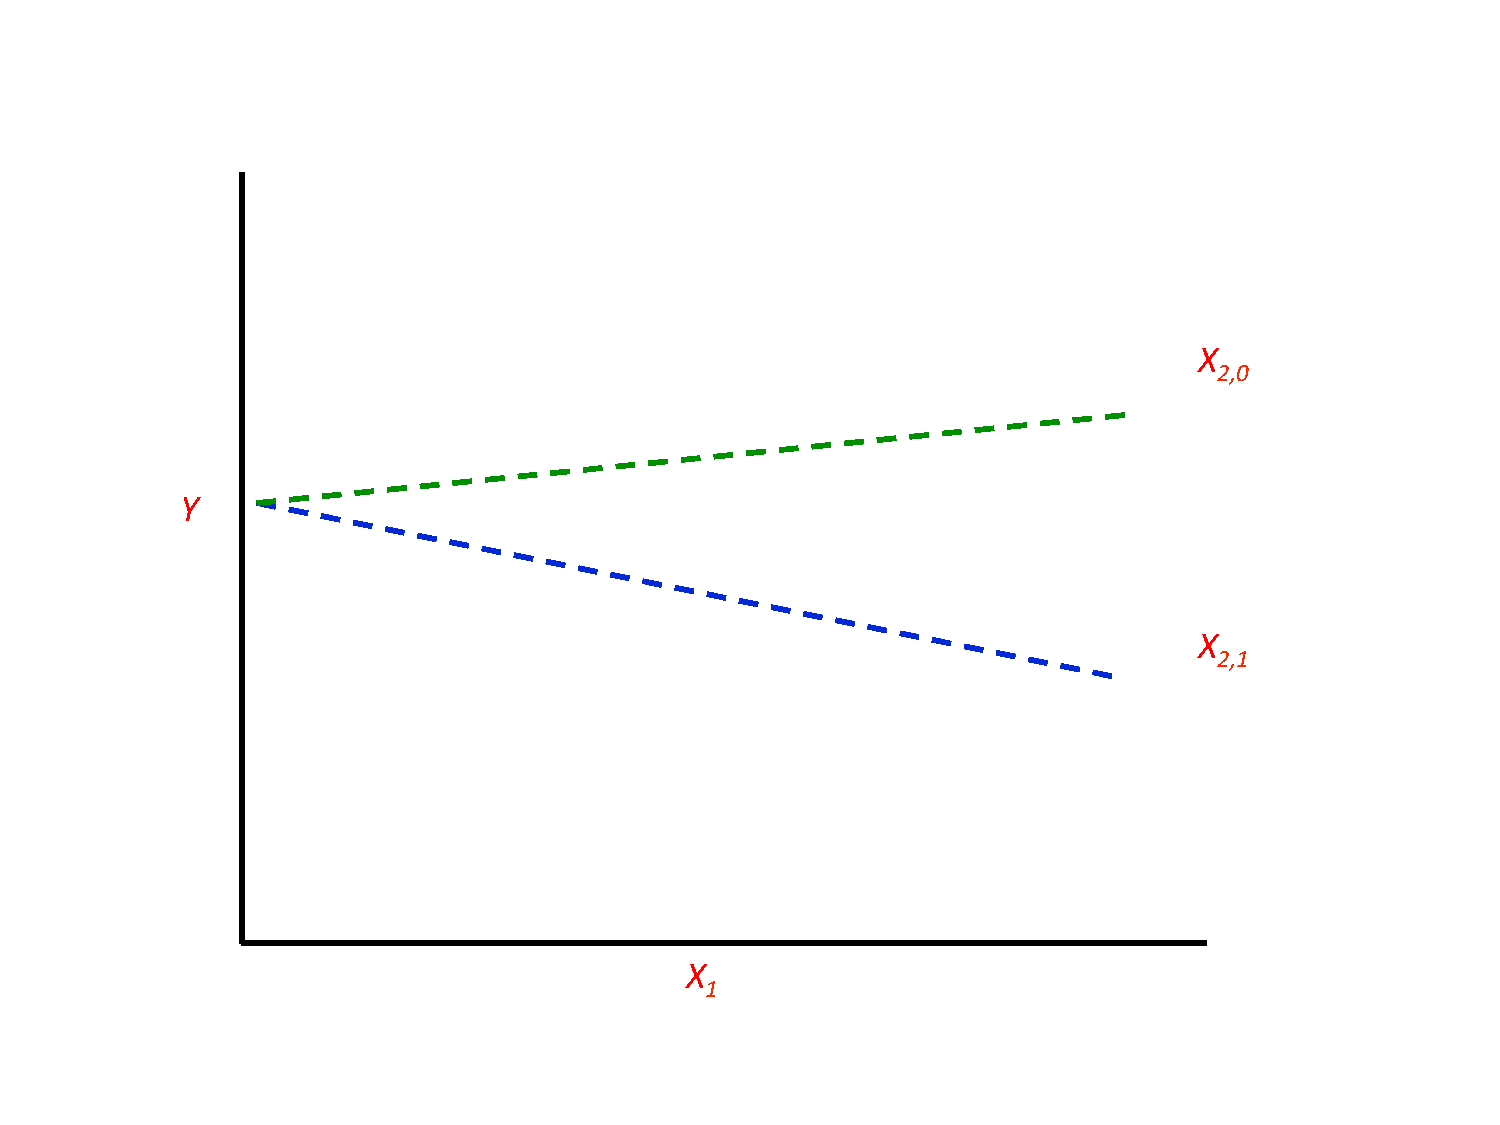
\includegraphics[width=5in]{../14_Topics/duminter.pdf}
  \caption {Illustration of Slope Interaction \label{fig:dumin}}
\end{figure}

We can test our hypothesized interaction in \texttt{R}, controlling for the effects of age
and income. 
\begin{knitrout}
\definecolor{shadecolor}{rgb}{0.969, 0.969, 0.969}\color{fgcolor}\begin{kframe}
\begin{alltt}
\hlstd{ols2} \hlkwb{<-} \hlkwd{lm}\hlstd{(glbcc_risk} \hlopt{~} \hlstd{age} \hlopt{+} \hlstd{income} \hlopt{+} \hlstd{education} \hlopt{+} \hlstd{gender} \hlopt{*} \hlstd{ideol,} \hlkwc{data} \hlstd{= ds.temp)}
\hlkwd{summary}\hlstd{(ols2)}
\end{alltt}
\begin{verbatim}
## 
## Call:
## lm(formula = glbcc_risk ~ age + income + education + gender * 
##     ideol, data = ds.temp)
## 
## Residuals:
##    Min     1Q Median     3Q    Max 
## -8.718 -1.704  0.166  1.468  6.929 
## 
## Coefficients:
##                Estimate Std. Error t value Pr(>|t|)    
## (Intercept)   1.060e+01  3.297e-01  32.153  < 2e-16 ***
## age          -4.137e-03  3.665e-03  -1.129  0.25919    
## income       -2.322e-06  9.069e-07  -2.561  0.01051 *  
## education     6.829e-02  2.992e-02   2.282  0.02258 *  
## gender        5.972e-01  2.987e-01   1.999  0.04572 *  
## ideol        -9.591e-01  3.894e-02 -24.628  < 2e-16 ***
## gender:ideol -1.750e-01  5.974e-02  -2.929  0.00343 ** 
## ---
## Signif. codes:  0 '***' 0.001 '**' 0.01 '*' 0.05 '.' 0.1 ' ' 1
## 
## Residual standard error: 2.427 on 2264 degrees of freedom
## Multiple R-squared:  0.3664,	Adjusted R-squared:  0.3647 
## F-statistic: 218.2 on 6 and 2264 DF,  p-value: < 2.2e-16
\end{verbatim}
\end{kframe}
\end{knitrout}
The results indicate a negative and significant interaction effect for gender and ideology. Consistent with our hypothesis, this means that the effect of ideology on climate change risk is more pronounced for males than females. Put differently, the slope of ideology is steeper for males than it is for females. This is shown in Figure \ref{fig:dummales}. 


\begin{figure}
  \centering
  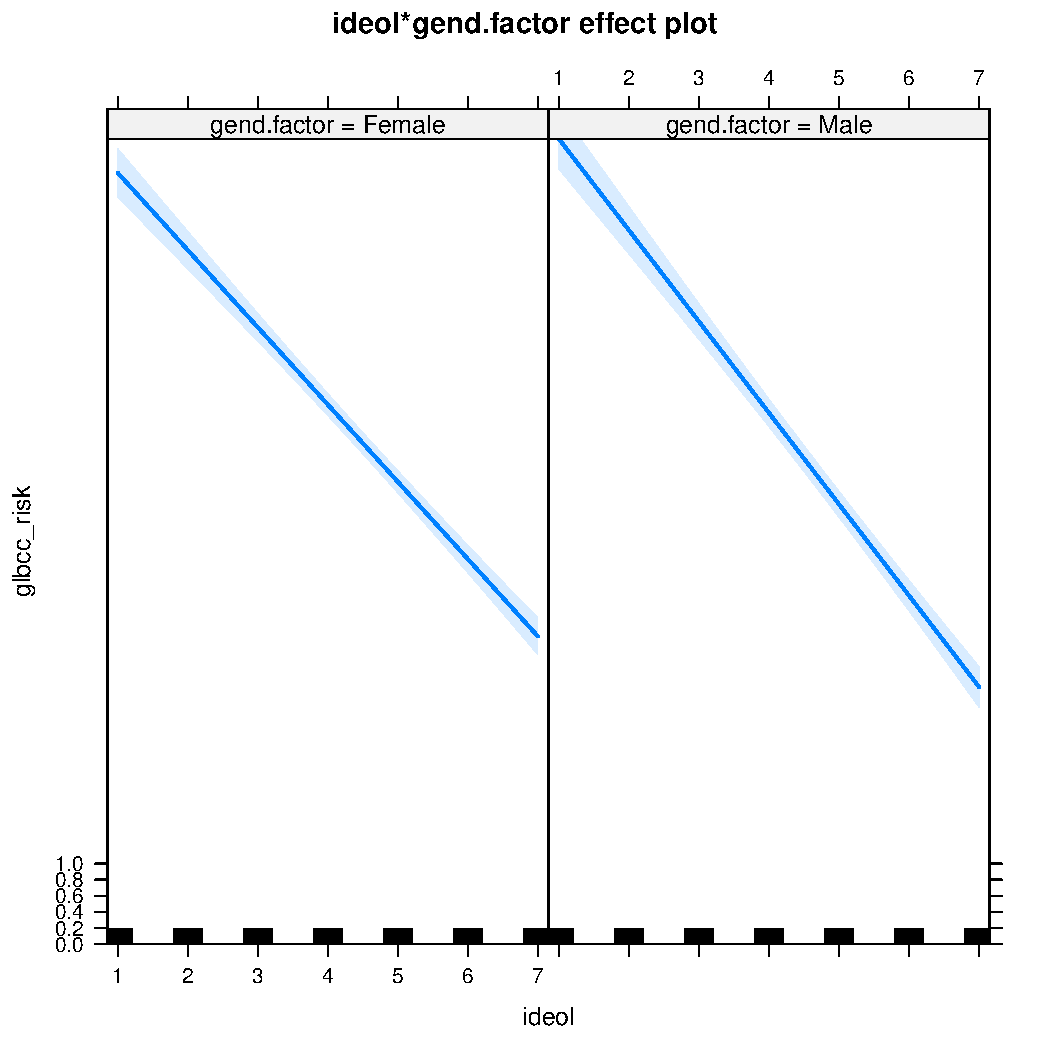
\includegraphics[width=4in]{../14_Topics/dummales.pdf}%filename
  \caption {Interaction of Ideology and Gender \label{fig:dummales}}
\end{figure}

%above graphic had to remove ,length=5in

In sum, dummy variables add greatly to the flexibility of OLS model specification. They permit the inclusion of categorical variables, and they allow for testing hypotheses about interactions  of groups with other IVs within the model. This kind of flexibility is one reason that OLS models are widely used by social scientists and policy analysts.

\section{Standardized Regression Coefficients} 

In most cases, the various IVs in a model are represented on different measurement scales. For example, ideology ranges from 1 to 7, while age ranges from 18 to over 90 years old. These different scales make comparing the effects of the various IVs difficult.  If we want to directly compare the magnitudes of the effects of ideology and age on levels of environmental concern, we would need to \textbf{standardize} the variables. 

One way to standardized variables is to create a $Z$-score based on each variable. Variables are standardized in this way as follows:
\begin{equation}
  Z_i = \frac{X_i-\bar{X}}{s_x} 
\end{equation}
\noindent where $s_x$ is the s.d. of $X$. Standardizing the variables by creating $Z$-scores re-scales them so that each variables has a mean of $0$ and a s.d. of $1$. Therefore, all variables have same mean and s.d. It is important to realize (and it is somewhat counter-intuitive) that the standardized variables retain all of the variation that was in the original measure.

A second way to standardize variables converts the unstandardized $B$, into a standardized $B'$. 
\begin{equation}
  B'_k = B_k\frac{s_k}{s_Y}  
\end{equation}
where $B_k$ is the unstandardized coefficient of $X_k$, $s_k$ is the s.d. of $X_k$, and $s_y$ is the s.d. of $Y$. Standardized regression coefficients, also known as beta weights or ``betas", are those we would get if we regress a standardized $Y$ onto standardized $X$’s. 
 
\begin{grbox}
\greybox{\textbf{Interpreting Standardized Betas}

\begin{itemize}  
\item The standard deviation change in $Y$ for a one-standard deviation change in $X$ 
\item All $X$’s on a equal footing, so can compare the strength of the effects of the $X$’s 
\end{itemize}  

\textbf{Cannot be used for comparisons across samples}
\begin{itemize}
\item Variances will differ across different samples
\end{itemize}}
\end{grbox}

We can use the \texttt{scale} function in \texttt{R} to calculate a $Z$ score for each of our variables, and then re-run our model. 
\begin{knitrout}
\definecolor{shadecolor}{rgb}{0.969, 0.969, 0.969}\color{fgcolor}\begin{kframe}
\begin{alltt}
\hlstd{stan.ds} \hlkwb{<-} \hlstd{ds.temp} \hlopt
  \hlkwd{select}\hlstd{(glbcc_risk, age, education, income, ideol, gender)} \hlopt
  \hlstd{scale} \hlopt
  \hlkwd{data.frame}\hlstd{()}

\hlstd{ols3} \hlkwb{<-} \hlkwd{lm}\hlstd{(glbcc_risk} \hlopt{~} \hlstd{age} \hlopt{+} \hlstd{education} \hlopt{+} \hlstd{income} \hlopt{+} \hlstd{ideol} \hlopt{+} \hlstd{gender,} \hlkwc{data} \hlstd{= stan.ds)}
\hlkwd{summary}\hlstd{(ols3)}
\end{alltt}
\begin{verbatim}
## 
## Call:
## lm(formula = glbcc_risk ~ age + education + income + ideol + 
##     gender, data = stan.ds)
## 
## Residuals:
##      Min       1Q   Median       3Q      Max 
## -2.92180 -0.54357  0.06509  0.48646  2.20164 
## 
## Coefficients:
##               Estimate Std. Error t value Pr(>|t|)    
## (Intercept)  1.685e-16  1.675e-02   0.000  1.00000    
## age         -1.877e-02  1.696e-02  -1.106  0.26865    
## education    3.957e-02  1.782e-02   2.220  0.02653 *  
## income      -4.669e-02  1.788e-02  -2.611  0.00908 ** 
## ideol       -5.883e-01  1.709e-02 -34.426  < 2e-16 ***
## gender      -3.592e-02  1.700e-02  -2.112  0.03475 *  
## ---
## Signif. codes:  0 '***' 0.001 '**' 0.01 '*' 0.05 '.' 0.1 ' ' 1
## 
## Residual standard error: 0.7984 on 2265 degrees of freedom
## Multiple R-squared:  0.364,	Adjusted R-squared:  0.3626 
## F-statistic: 259.3 on 5 and 2265 DF,  p-value: < 2.2e-16
\end{verbatim}
\end{kframe}
\end{knitrout}

In addition, we can convert the original unstandardized coefficient for ideology, to a standardized coefficient. 
\begin{knitrout}
\definecolor{shadecolor}{rgb}{0.969, 0.969, 0.969}\color{fgcolor}\begin{kframe}
\begin{alltt}
\hlstd{sdX} \hlkwb{<-} \hlkwd{sd}\hlstd{(ds.temp}\hlopt{$}\hlstd{ideol,} \hlkwc{na.rm}\hlstd{=}\hlnum{TRUE}\hlstd{)}
\hlstd{sdY} \hlkwb{<-} \hlkwd{sd}\hlstd{(ds.temp}\hlopt{$}\hlstd{glbcc_risk,} \hlkwc{na.rm}\hlstd{=}\hlnum{TRUE}\hlstd{)}
\hlstd{ideology.prime} \hlkwb{<-} \hlstd{ols1}\hlopt{$}\hlstd{coef[}\hlnum{5}\hlstd{]}\hlopt{*}\hlstd{(sdX}\hlopt{/}\hlstd{sdY)}
\hlstd{ideology.prime}
\end{alltt}
\begin{verbatim}
##      ideol 
## -0.5882792
\end{verbatim}
\end{kframe}
\end{knitrout}

Using either approach, standardized coefficients allow us to compare the magnitudes of the effects of each of the IVs on $Y$.

\section{Summary}
This chapter has focused on options in designing and using OLS models. We first covered the use of dummy variables to capture the effects of group differences on estimates of $Y$. We then explained how dummy variables, when interacted with scale variables, can provide estimates of the differences in how the scale variable affects $Y$ across the different subgroups represented by the dummy variable. Finally, we introduced the use of standardized regression coefficients as a means to compare the effects of different $Xs$ on $Y$ when the scales of the $Xs$ differ. Overall, these refinements in the use of OLS permit great flexibility in the application of regression models to estimation and hypothesis testing in policy analysis and social science research.


\end{document}
